\chapter{Описание алгоритмов}
\label{ch:chap1}

\section{K-RLE}

В контексте использования технологии беспроводной сенсорной сети
(WSN) для мониторинга окружающей среды двумя
основными элементарными функциями WSN являются сбор
и передача данных. Однако передача/прием данных
требует больших затрат энергии. Чтобы снизить энергопотребление, связанное с передачей, используется сжатие данных с помощью локальной обработки информации.

Рассмотрим новый алгоритм сжатия данных, основанный на кодировании длины выполнения (RLE), который называется K-RLE.

Идея, лежащая в основе этого нового алгоритма, заключается в следующем:
пусть $K$ - число, если элемент данных $d$, $d+K$ или $d-K$ встречается n раз подряд во входном потоке, мы заменяем эти n вхождений
одной парой $nd$ \cite{krle_article}.

\begin{figure}[ht]
    \centering
    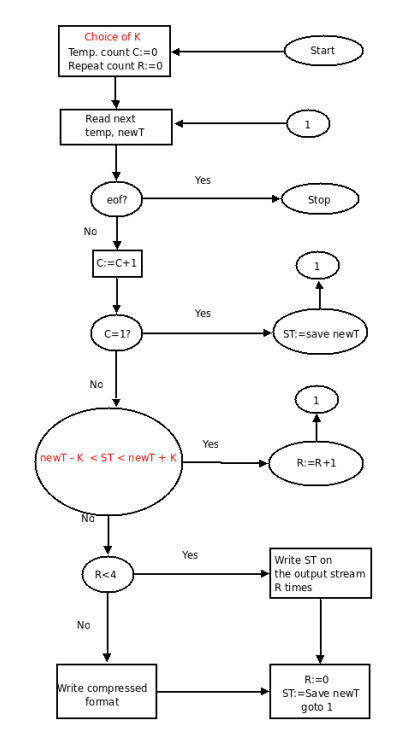
\includegraphics[width=0.5\textwidth]{krle_alg.png}
    \caption{K-RLE Алгоритм}
    \label{fig:krle_alg}
\end{figure}

\section{LTC}

Алгоритм LTC (легковесное кодирование), использует линейность во времени
для сжатия данных. Наш метод аналогичен кодированию по
длине цикла (RLE) в том смысле, что мы пытаемся
представить длинную последовательность схожих данных с
помощью одного символа. Если при кодировании длины выполнения выполняется поиск строк
с повторяющимся символом, мы ищем линейные тренды.
Пусть ri = (ti, vi) - точка выборки с допустимой
погрешностью e. Исходный набор данных R = r0, r1, ..., rj
преобразуется в поток обработанных точек, S =
s0, s1, ..., sk, где k ≤ j (обычно k ≤≤ j). Пусть
L = l0, l1, ..., lk−1 - набор отрезков, таких, что
li - это отрезок прямой, соединяющий две точки si и
si+1. Кусочно-непрерывная функция, определяемая
отрезками из L, аппроксимирует R таким образом, что ни одна точка в
R не находится на расстоянии более e от ближайшего
отрезка прямой в L по вертикали \cite{ltc_article}. \\

Алгоритм: 
\begin{enumerate}
    \item Инициализация: Получаем первую точку данных, сохраняем в z. Получаем следующую точку данных (t2, v2), используем ее для инициализации пределов UL (для UL задано значение (t2, v2 + e)) и LL (для LL задано значение (t2, v2 − e)).
    \item Вычислите верхнюю линию, которая будет линией, соединяющей z и UL.
    \item Вычислите нижнюю линию, которая будет линией, соединяющей z и LL.
    \item Получите следующую точку данных. Преобразуйте точку в вертикальный сегмент, используя поле e. Пусть ul - самая высокая точка отрезка. Пусть ll - самая низкая точка отрезка.
    \item Если верхняя линия находится ниже ll или нижняя линия находится выше ul, перейдите к пункту 9, в противном случае переходите к следующему шагу
    \item Если верхняя строка выше ul, то установите значение UL равным ul.
    \item Если нижняя строка ниже ll, то установите значение LL равным ll.
    \item Переход ко второму этапу.
    \item Снимите заглушку: выведите z в поток выходных данных.
    \item Установите точку z на полпути между UL и LL.
    \item Установите значение UL равным ul.
    \item Установите значение LL равным lll.
    \item Переход ко второму этапу
\end{enumerate}


\endinput